%%%%%%%%%%%%%%%%%%%%%%%%%%%%%%%%%%%%%%%%%%%%%%%%%%%%%%%%%%%
%
%		Relazione del progetto di Gestione di Rete
%
%		    Nicola Corti & Michael Sanelli - 2011
%
%%%%%%%%%%%%%%%%%%%%%%%%%%%%%%%%%%%%%%%%%%%%%%%%%%%%%%%%%%%
\documentclass[a4paper, 10pt]{article}

\usepackage{graphicx}
\usepackage[italian]{babel} 
\usepackage[latin1]{inputenc}

\title{\texttt{SNMPTweet} - demone per la ricezione di trap e la notifica su
Twitter}
\author{Nicola Corti - Michael Sanelli \\Corso di Laurea in Informatica
(L-31) - Universit\`a di pisa}
\date{12 Settembre 2011}


\begin{document}
\maketitle

\begin{abstract}
Questa relazione ha lo scopo di illustrare i dettagli implementativi, le scelte
che sono state prese, e le metodologie di programmazione utilizzate nello
sviluppo di \texttt{SNMPTweet}.
\end{abstract}

\tableofcontents

\newpage

\section{Introduzione}
\texttt{SNMPTweet} \`e un demone che permette di ricevere le trap SNMP, di elaborarle e di pubblicarle sul social network Twitter (http://www.twitter.com).
Le trap SNMP, secondo quanto descritto all'interno dell'RFC 1157, rappresentano messaggi asincroni normalmente utilizzati per indicare eventi o errori che si sono manifestati e a cui \`e necessario prestare attenzione.

L'utente pu\'o configurare il proprio agent SNMP per inviare le trap al calcolatore dove \`e in esecuzione \texttt{SNMPTweet}, il quale elaborer\`a la coda delle trap ricevute e le invier\`a come Tweet su Twitter, secondo le modalit\'a decise dall'utente nel file di configurazione.

\section{Dettagli implementativi e scelte prese}

Segue una breve panoramica dell'architettura del sistema, le scelte che sono state prese e le motivazioni che ci hanno spinto a prenderle.

I dettagli descritti in questa sezione, servano d'ausilio ai programmatori che vogliano comprendere maggiormente la logica applicativa.

\subsection{Architettura generale dell'applicativo}

L'applicativo \`e stato sviluppato in Java, cos\`i da poter essere compatibile con tutte le piattaforme che supportino la JVM.

L'utilizzo di Java va  per\`o a discapito delle performance del software, che risultano inferiori rispetto ad una possibile realizzazione del software con un linguaggio pi\`u a basso livello (ad esempio C).

Abbiamo deciso di strutturare il nostro sistema in modo modulare, cos\`i da favorire una futura espandibilit\`a. L'utilizzo di un linguaggio di programmazione a oggetti ci ha aiutato in questo intento, in particolar modo abbiamo utilizzato i \texttt{package} di Java.

I package che abbiamo realizzato sono:
\begin{itemize}
	\item \texttt{twitter} che si occupata dell'interfacciamento con Twitter;
	\item \texttt{snmptrap} che si occupa di ricevere e leggere le trap SNMP;
	\item \texttt{intracomunication} che contiene gli strumenti per gestire una o pi\`u code di trap.
\end{itemize}

Abbiamo utilizzato inoltre alcune librerie:
\begin{description}
	\item[Java SNMP\footnote{http://gicl.cs.drexel.edu/people/sevy/snmp/}] che implementa il protocollo SNMP;
	\item[Twitter4J\footnote{http://twitter4j.org/}] che implementa le API di Twitter;
	\item[Mibble\footnote{http://mibble.org/}] che implementa un semplice parser per i MIB Files;
	\item[Log4j\footnote{http://logging.apache.org/log4j/}] che fornisce gli strumenti per gestire i file di log.
\end{description}

Segue una rappresentazione grafica dell'architettura del sistema:

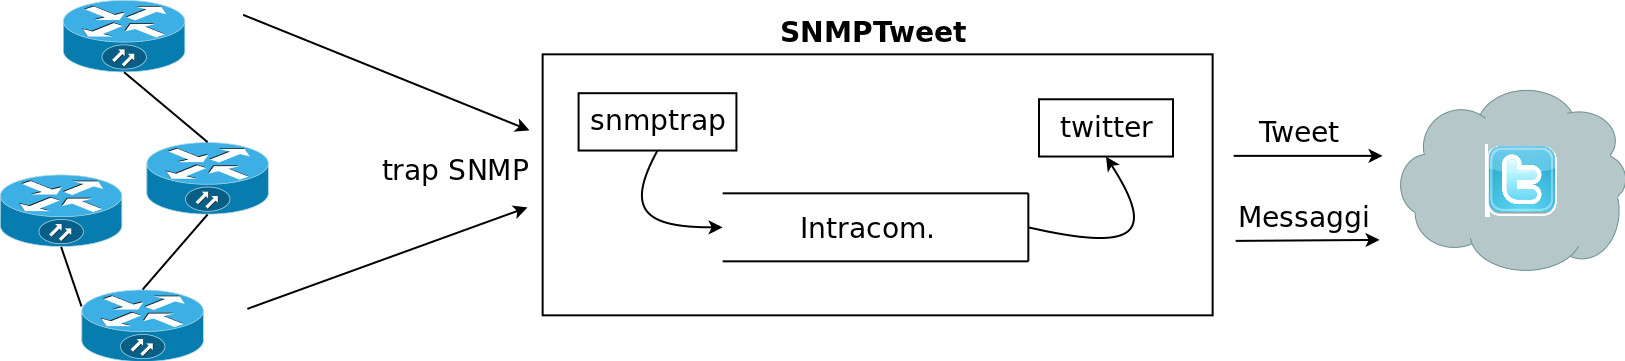
\includegraphics[scale=0.20]{diagram.png}

\subsection{Ricezione di trap SNMP}

La ricezione delle trap \`e affidata alle classi contenute nel package \texttt{snmptrap}.

In particolar la classe \texttt{ListenTrapV1} implementa \texttt{SNMPv1TrapListener}, interfaccia definita nella libreria Java SNMP, che ci permette di definire un listener per le trap in entrata. All'interno di questa classe abbiamo definito il comportamento che il software deve avere all'atto della ricezione di una trap: ogni volta che viene ricevuta una trap, viene creato un nuovo oggetto all'interno del quale vengono inseriti i dati della trap e l'oggetto viene accodato per essere processato.

La classe \texttt{TrapReceiver} permette di inizializzare l'interfaccia di ascolto delle trap e di iniziarne la ricezione.

\subsubsection{Ricerca di OID tra i MIB file}

La classe \texttt{MibParser} implementa un piccolo parser per i file di Mib.
Abbiamo deciso di realizzare il parser mediante un vettore di oggetti di tipo \texttt{Mib}, al quale si accede grazie ad un iteratore, e che permette di convertire un OID nella stringa della sua descrizione.

Grazie ai metodi contenuti nella classe \`e possibile:
\begin{itemize}
	\item Caricare in memoria tutti i Mib da una directory settata fra le configurazioni.
	\item Convertire da un OID a Stringa, ricercando fra i Mib precedentemente caricati.
\end{itemize} 

\subsection{Interfacciamento con Twitter}

La gestione dell'interfaccia con Twitter viene gestita dal package \texttt{twitter}.

La classe \texttt{MyTwitter} contiene tutti i metodi per potersi interfacciare in modo corretto con Twitter. Il metodo \texttt{HandShaker} consente di effettuare il login su twitter con l'account desiderato; nel caso in cui l'utente non abbia mai utilizzato in precedenza il software, verr\`a chiesto all'utente di visitare una pagina web per poter effettuare il login, una volta autenticato correttamente, i dati di accesso verranno memorizzati in modo da non dover pi\`u ripetere tale procedura.

Con il metodo \texttt{sendUpdate} \`e possibile inviare tweet o messaggi privati su Twitter in base alla configurazione. Il metodo si occupa anche di gestire tweet pi\`u lunghi di 140 caratteri.

Il metodo \texttt{ExceptionHandler} consente di gestire tutti gli eventuali problemi che potrebbero sorgere nell'autenticazione o nell'invio dei tweet (Twitter impone infatti varie limitazioni sul numero dei tweet che possono essere inviati), analizzando il codice della risposta http ricevuta da Twitter.

\subsubsection{Gestione dell'autenticazione}

Per il processo di autenticazione viene utilizzato il protocollo \texttt{OAuth}, che risulta il pi\`u sicuro fra i protocolli disponibili per l'autenticazione su twitter.

Per la gestione delle chiavi abbiamo utilizzato la classe \texttt{KeyContainer}, che funge da ""contenitore'' per le chiavi: sia per quelle legate al software, sia quelle legate all'utente.

Abbiamo utilizzato la serializzazione per rendere le chiavi persistenti, e per un minimo livello di sicurezza. Per rendere pi\`u sicura la gestione delle chiavi, avremmo potuto cifrare il contenuto del file.

\subsection{Logfile e Config file}

Ogni operazione eseguita dal software viene registrata all'interno di un file di log, gestito grazie alla libreria \texttt{log4j}. In questo modo l'utente pu\`o capire meglio quali problemi sono avvenuti o quali tweet sono andati persi.

Abbiamo inoltre deciso di fornire all'utente un file di configurazione (il file ""./snmptweet.conf'') in modo da poter configurare a piacimento le varie funzionalit\`a che andremo ad elencare qua sotto:

\begin{description}
	\item[LOG\_FILE] il nome del file di log,
	\item[MIB\_DIR] la directory dei Mib,
	\item[PORT] la porta di ascolto delle trap SNMP,
\end{description}

Inoltre settendo il valore del parametro \texttt{PRIVATE} a true (di default il valore \`e false), verranno inibiti tutti gli invii di tweet pubblici. In questo modo verranno inviati soltanto messaggi privati. Se si imposta \texttt{PRIVATE} a true, \`e necessario configurare inoltre le associazioni fra utenti di Twitter e indirizzi IP dell'agent che ha inviato la trap.

Tali associazioni si possono impostare mediante l'inserimento di coppie del tipo $(USER_i, IP_i)$. Nel caso in cui non sia settata la modalit\`a \texttt{PRIVATE}, ma siano state settate delle associazioni, verr\`a inviato un tweet pubblico, e verr\`a inviato inoltre un messaggio privato all'utente relativo.

\section{Possibili sviluppi futuri}

Il software \`e stato sviluppato in un'ottica da poter permettere eventuali miglioramenti futuri, grazie alla sua architettura modulare, e alla sua suddivisione in pacchetti.

Presentiamo alcuni dei possibili miglioramenti che potrebbero essere implementati nelle versioni successive:

\begin{itemize}
	\item Possibilit\`a di interrogare i dispositivi, o di modificare le loro configurazione con delle \texttt{GET/SET SNMP} mediante dei messaggi privati inviati all'utente collegato a snmp-tweet.
	\item Possibilit\`a di impostare varie tipologie di filtri per limitare la ricezione delle \texttt{TRAP}.
	\item Possibilit\`a di impostare la modalit\`a privata o pubblica in modo separato per ogni dispositivo.
	\item Possibilit\`a di impostare la geo-localizzazione dei dispositivi che emettono trap e di corredare i tweet delle informazioni geografiche.
	\item Possibilit\`a di gestire pi\`u di un account twitter contemporaneamente.
	\item Possibilit\`a di impostare pi\`u porte sul quale ricevere le \texttt{TRAP}.
	\item Possibilit\`a di ricevere \texttt{TRAP} versione 2 e 3 e le \texttt{INFORM}.
\end{itemize}

\section{Installazione del software}

Il software \`e corredato di un file \texttt{ant} per l'automazione del processo di installazione.

Per creare il \texttt{jar} eseguibile \`e sufficiente invocare il comando 
\begin{center}
\texttt{ant makejar}
\end{center}
nella directory root del progetto. Cos\`i facendo, troverete il file \texttt{jar} all'interno della directory \texttt{dist}. Per eseguire il software \`e sufficiente invocare il comando:

\begin{center}
	\texttt{java -jar SNMPTwitter.jar}
\end{center}

Se invece si \`e interessati a compilare i file binari, \`e sufficiente invocare il comando \texttt{ant}. I file binari si troveranno dentro la directory \texttt{bin}.


\section{Documentazione allegata}

Tutto il codice sorgente scritto \`e corredato di commenti che descrivono i dettagli implementativi del software.

Inoltre \`e stato scritto il javadoc dell'intero progetto, in modo da poter aiutare i programmatori nella comprensione dell'organizzazione logica delle classi.

Per ricreare il javadoc \`e sufficiente utilizzare il target \texttt{javadoc} del file ant.

\`E stato inoltre scritto il file README destinato all'utente che non vuole conoscere i dettagli implementativi, ma che lo pu\`o aiutare nella configurazione del sistema e nella risoluzione dei problemi.

\section{Licenza d'uso}
Snmp-tweet \`e rilasciato sotto licenza libera, in modo che ogni utente sia libero di poterlo modificare e ridistribuirlo liberamente.

In particolare \`e stato rilasciato sotto licenza GNU GPL (General Public Licence) v.3: 
\begin{verbatim}
snmp-tweet is free software: you can redistribute it 
and/or modify it under the terms of the GNU General 
Public License as published by the Free Software Foundation,
either version 3 of the License,
or (at your option) any later version.

snmp-tweet is distributed in the hope that
it will be useful, but WITHOUT ANY WARRANTY;
without even the implied warranty of MERCHANTABILITY
or FITNESS FOR A PARTICULAR PURPOSE.  See the
GNU General Public License for more details.

You should have received a copy of the GNU General 
Public License along with Foobar. 
If not, see <http://www.gnu.org/licenses/>.
\end{verbatim}

\end{document}
